\section{Аналитическая часть}
Необходимо разработать метод, который по заданной информации об элементах транспортной системы формировал бы рекомендации по объёмам и маршрутам поставки.

\subsection{Актуальность проблемы}
	В данный момент торговые розничные сети (другое название -- ретейл) динамически развиваются и с каждым годом занимают всё большую долю в общем объёме розничной торговли\cite{subj:demand}. Деятельность подобных предприятий тесно связана с управлением цепочками поставок (SCM -- Supply Chain Management) -- комплекс подходов, помогающий эффективной интеграции поставщиков, производителей, дистрибьюторов
	и продавцов. Этот процесс можно разделить на следующие этапы\cite{subj:scm}. 
	\begin{enumerate}
		\item Планирование. Принимается решение об управлении жизненным циклом товаров, объёмах производства и закупок.
		\item Закупки. Происходит управление снабжением, оцениваются и выбираются поставщики.
		\item Производство. Включает в себя процесс производства, контроль технологических изменений, управление качеством и т.д.
		\item Доставка. Состоит из трёх основных процессов: управление заказами, управление складом и транспортировка.
		\item Возврат. На этом этапе определяются элементы возврата товара, составляются графики возврата и направления на уничтожение и переработку.
	\end{enumerate}
	
	Среди данных задач хочется выделить отдельно транспортную логистику. Затраты на неё являются существенными, что обосновывается её сложностью и жизненной важностью для деятельности фирмы. 
	
	Таким образом, расширение сегмента розничных сетей на рынке влечёт за собой повышение спроса на перевозку товаров. Большинство транспортных компаний прибегают к использованию программного обеспечения для ускорения и упрощения различных этапов процесса перевозки\cite{subj:auto_eff}.  Автоматизация данной работы позволяет повысить её эффективность и надёжность.

\subsection{Анализ предметной области}
	Целью деятельности транспортной логистики является организация перемещения груза между двумя местами по оптимальному маршруту\cite{subj:main}. В данном случае оптимальным считается тот маршрут, который позволяет перевезти объекты в предусмотренные сроки (желательно, минимальные) с наименьшими затратами и вредом для них. Стоит отметить, что зачастую возможные маршруты не являются оптимальными сразу по всем критериям, поэтому приходится принимать компромиссные решения.
	
	Случаи, когда задачи розничной торговли, транспортировки и складирования товара (а иногда даже производства) выполняются одной фирмой достаточно редки и характерны только для крупного бизнеса. Этот подход организации позволяет улучшить интеграцию всех перечисленных элементов логистической системы, что способно снизить издержки на каждом из этапов. Малые предприятия не располагают подобными ресурсами и, как правило, пользуются услугами других компаний для данной функции.  
	
	В рамках данной работы рассматривается решение задач автоматического планирования для автомобильной транспортной компании.
	
	Логистика малого бизнеса имеет ряд особенностей\cite{subj:small_business}. Как было отмечено, небольшие организации не способны содержать необходимый штат сотрудников, транспортных средств и т.д., а также не обладают достаточно большим оборотом товаров для собственной организации перевозки. Малые объёмы поставок для каждого отдельного предприятия приводят к тому, что компании-перевозчики совмещают планируют один маршрут сразу через несколько точек доставки.
	
	Можно заключить, что обыкновенный процесс работы фирмы доставки заключается в следующем. Несколько ретейл-предприятий формируют заказы с указанием заказываемых товаров и их объёмов. Транспортная компания определяет совместные маршруты и средства доставки, формирует заказ для складского предприятия. Назначенные грузовые автомобили загружаются на складе и развозят груз по нужным пунктам.

\subsection{Сравнение с аналогами}
	Системы управления перевозками (TMS -- Transportation management system), как было отмечено выше, являются востребованными для предприятий, занимающихся логистикой. Данные системы, в основном, решают следующий перечень задач\cite{subj:tms_cmp}:
	\begin{itemize}
		\item расчет логистических затрат;
		\item оптимальное использование транспортных средств для минимизации
		общих расходов;
		\item повышение качества обслуживания -- соблюдение сроков доставки, установленных транспортной службой компании;
		\item автоматизация процесса транспортного планирования и управления,
		обеспечивающая решение для конкурентного транспортного планирования
		и управления;
		\item повышение производительности труда работников при планировании и
		организации грузовых перевозок.
	\end{itemize}

	\hfill
	
	В число наиболее популярных в России входят следующие TMS.
	\begin{itemize}
		\item Oracle Transportation Management.
		\item SAP TM.
		\item 1С: TMS Логистика. Управление перевозками.
	\end{itemize}

	Перечисленные программы позволяют осуществлять составление, расчёт стоимостей, поручение и контроль выполнения транспортировок. Также зачастую реализуются различные интерфейсы и функционал для водителей, логистов и т.д. Таким образом, общей чертой данных систем является комплексный подход к решению задач транспортной логистики. Предпринимается попытка удовлетворить все потребности, так или иначе связанные с обработкой данных. Сравнение наиболее интересных для данной задачи функций\cite{subj:tms_cmp} можно привести в таблице \ref{cmp_table}.
	
	\begin{table}[h]
		\begin{center}
			\caption{Сравнение существующих решений}
			\label{cmp_table}
			\begin{tabular}{| p{5cm} | p{2.5cm} | p{2.5cm} | p{2.5cm} |}
				\hline
				\backslashbox{\textbf{Функция}}{\textbf{TMS}} &
				OTM &
				SAP &
				1C \\
				
				\hline
				Прогнозирование & 
				да &
				да &
				нет \\
				 
				\hline
				Планирование заказов &
				да &
				частично &
				частично \\
				
				\hline
				Распределение перевозок между исполнителями за период &
				да &
				да &
				нет \\
				
				\hline
			\end{tabular}
		\end{center}
	\end{table}
	
	Однако среди указанных программ автоматическое планирование с учётом наиболее важных факторов позволяет Oracle TM. В случае других TMS планирование не реализовано настолько детально. Ввиду крайне высокой цены\cite{subj:tms_cmp} на Oracle Transportation Management и в целом на подобные программы, небольшие транспортные фирмы не могут позволить себе столь высокие расходы. Решением может быть использование представленной в этой работе программой в интеграции с сравнительно недорогой TMS, решающей другие задачи транспортного управления.
	

\subsection{Детализация задачи}
	Требуется разработать алгоритм, выполняющий оптимальную планировку маршрутов доставки заказов от складов до потребителей (ретейл-фирм). Целью создания продукта является определение маршрутов, которые будут наиболее выгодными для компании. Выгода в данном случае заключается во множестве факторов, но в первую очередь под ней подразумевается денежная прибыль.
	
	Целевой пользователь -- логист транспортной компании. Для него применение программы нужно для получения рекомендаций по заданию маршрутов в определённый момент времени. После этого работник может проанализировать полученные маршруты, внести в них свои корректировки и заняться последующими этапами своей деятельности (непосредственно организации грузоперевозок, документооборотом и т.д.).
	
	Исходными данными является информация о следующих объектах:
	\begin{itemize}
		\item грузовые машины, входящие в автопарк фирмы;
		\item перевозимые товары;
		\item стоянка грузовиков;
		\item поставщики и потребители товара (в данном случае склады и розничные торговые фирмы);
		\item пути между вышеописанными пунктами маршрута;
		\item заказы.
	\end{itemize}

	Результатом работы должны стать предлагаемые маршруты. Схематически пример модели представлен на рисунке \ref{pic:model}, где стрелками обозначены маршруты, выбранные алгоритмом как оптимальные.
	
	\begin{figure}[h!] 
		\begin{center}
			{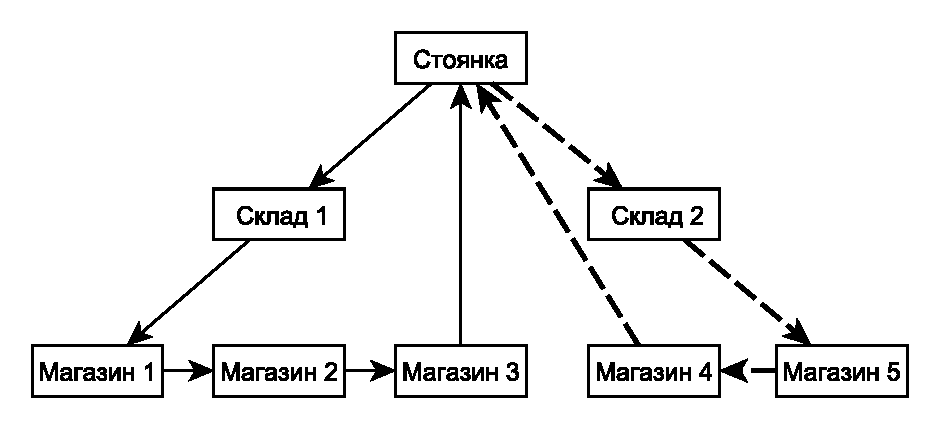
\includegraphics[scale=0.9, angle=0]{img/model.pdf}}
			\caption{Схема модели}
			\label{pic:model}
		\end{center}
	\end{figure}
	
	\subsection{Допущения и ограничения задачи}
	Рассмотрим упомянутые объекты, обозначим допущения и ограничения для задачи.
	
	Одним из главных вопросов является выделение критерия оптимизации, служащего для оценки решений. Как было отмечено выше, главным является денежная прибыль, то есть повышение доходов и уменьшение затрат.   
	
	Первый путь достигается только через выполнение большего объёма грузоперевозок. Однако, количество перевозимого груза определяется не при планировании маршрутов перевозки товаров, а при заключении договора между транспортной компанией и ритейл-фирмой. Поэтому, будем считать, что объём заказов фиксирован и их выполнение в срок является обязательным. Это также обусловленно большими штрафами за невыполнение договора, как правило существенно превышающими рассмотренные далее затратами.
	
	Деятельность фирмы грузодоставки связана с множеством статей затрат, но пути перевозки влияют только на время доставки и пробег грузовиков, что в свою очередь отражается на средствах, затрачиваемых на топливо и амортизацию транспортных средств. Для упрощения, будем считать, что этот расход можно вычислить используя длину маршрута и среднюю затрату на километр. Оценка по времени для расчёта стоимости подходит меньше, так как одинаковое время затраченное в пробке и на свободной дороге ведёт к совершенно разным результатам.
	
	Путь между пунктами доставки достаточно описать с использованием расстояния и времени. Следует уточнить, что последний фактор является крайне динамичным, ввиду разной загруженности дорог в разные периоды суток, возможностью ДТП и прочих сложно прогнозируемых событий. Поэтому время должно указываться  усреднённое за весь период дня. Также в расчёте времени, затрачиваемого на рейс, следует учитывать продолжительность загрузки и выгрузки товаров, а также интервалов между разными заказами. Эти параметры зависят от большого количества факторов. Также время не является целью оптимизации в данной работе и служит только для задания ограничения. Поэтому данные величины могут быть заданы постоянными.
	
	Таким образом, продолжительность рейса может быть рассчитанна как сумма длительности всех путей и постоянных на перенос грузов.
	
	Решение проблемы расположения разнородного груза в автомобиле и расчёта его вместимости в общем случае является достаточно затруднительным. Так, например, хрупкие вещи могут не допускать расположение другого груза поверх них. Поставка товаров является оптовой в поставленной задаче, поэтому примем распространённый в этой сфере подход: все виды товаров поставляются в внутри тар, которые имеют определённый объём и не требуют специальных условий транспортировки. В таком случае также можно считать, что грузовик вмещает некоторые тары, если их суммарный объём не превышает заполняемый объём кузова.
	
	Для упрощения решаемой задачи следует также принять, что грузовики и перевозимые тары обладают одинаковой вместимостью и объёмом соотвественно. Транспортные фирмы зачастую действительно закупают или арендуют грузовые автомобили одной модели или разных, но со схожими характеристиками. Это объясняется тем, что они закупаются для одной целей, а также упрощением процедуры технического обслуживания одинаковых авто. Таким образом, данное упрощение существенно не влияет на применимость метода к реальным системам.
	
	Допущение о одинаковости тар сделано для упрощения разрабатываемого метода. Как было отмечено выше, форма и объём тар достаточно разнообразны, и их учёт повысит сложность и комплексность метода. Поэтому в качества объёма тар устанавливается одно значение. Для иных типов следует применять перевод их количества с сохранением общего объёма продукции. 
	
	Первым и последним пунктом любого рейса является автостоянка транспортной фирмы, причём в обоих случаях машина не содержит каких-либо грузов. Также будем считать, что в каждом маршруте склад посещается однократно. Это условие нужно для избежания длинных рейсов с промежуточными пополнениями.

\subsection{Формализация задачи}
	Сформулированная задача является задачей поиска оптимального решения, а именно транспортной задачей \cite{trans:main}. Она решает проблему составления плана перевозок из пунктов отправления в пункты потребления, который будет иметь наименьшие затраты на перевозки. 
	
	В простейшем случае модель транспортной системы рассматривается как множество пунктов производства однородного продукта и множество его потребителей. Известны затраты перевозки одной единицы товара для любой пары производителя и потребителя.
	
	Использование такой модели для решения поставленной задачи некорректно, так как она не учитывает следующие факторы.
	\begin{itemize}
		\item Склады и транспортные средства ограничены и обладают конечной вместимостью.
		\item Рассматриваемый магазин оперирует сразу множеством товаров. Это порождает сразу ряд дополнительных обстоятельств. Например, тары имеют различные габариты, что влияет на вместимость транспортного средства.
		\item Рассматриваются только маршруты "Производитель -- Потребитель"\, тогда как в рассмотренной модели маршрут может проходить сразу через несколько потребителей. Таким образом и перевозимый одним транспортом груз зависит сразу от нескольких потребителей.
	\end{itemize}
		
	Основным способом решения вопроса множества продуктов сводится к условному разбиению поставщиков и потребителей из общих на работающих только с одним продуктом. Таким образом задача сводится к множеству однопродуктовых, но с общим набором рейсов, что накладывает совместные ограничения.
	
	В таком случае рассмотрим математическую модель транспортной задачи для одного продукта.
	\paragraph{Формализация данных}
	Формализуем данные метода. В первую очередь обозначим основные величины: $Vol$ -- объём одной тары, $Con$ -- стоимость топлива (литр / у.е.)
	
	$A_i$ -- склады с запасом продукции в $a_i$, ($i = \overline{1, N_a}$).
	
	$B_i$ -- потребители с потребностью продукции в $a_i$, ($i = \overline{1, N_b}$).
	
	Данные об $A$ и $B$ и автостоянке можно объединить в понятие пункта маршрута $P$, где $a_i$ -- количество продукта (в случае потребителя отрицательно, по модулю равно потребности, для стоянки -- всегда 0), где $i = 1$ -- автостоянка $i = \overline{2, N_a + 1}$ -- склады, $i = \overline{N_a+2, N_b+N_a+1}$ -- потребители. Общее количество пунктов опишем как $N_P= N_b+N_a+1$.
	
	Дороги, связывающие пункты описываются с помощью параметров $t_{ij} > 0, d_{ij} > 0$ -- время перемещения и расстояние между $P_i$ и $P_j$.
	
	$Prod_i$ -- продукт ($i = \overline{1, N_{prod}}$).
	
	$O_i$ -- начальный баланс товаров в $i$-м пункте. $O_ij$ - баланс продукта $Prod_j$ в пункте $P_i$. Баланс характеризует дефицит или профицит товаров для определённого пункта. В случае, если пунктом является склад, то за баланс принимается объём запасов. Если это потребитель, то балансом считается заказ со знаком минус. Фактически решением задачи будет являться перераспределение продуктов так, чтобы во всех пунктах был неотрицательный баланс. 

	$T_i$ -- транспорт с вместимостью в $c$ (в кубометрах) и затратой топлива в $f$ (в литр / км) ($i = \overline{1, N_t}$). Как было сказано ранее, в данной задаче все грузовики обладают одинаковыми характеристиками.
	
	Рейсы обозначим как $R_i$ ($i = \overline{1, N_R}$). $RT_i = \overline{1, N_t}$ -- индекс транспорта, назначенного на $i$-й маршрут.
	
	$RP_i$ - вектор пунктов, задействованных в $i$-м рейсе. $RP_i[j]$ - индекс пункта, посещённый в $j$-ю очередь на $i$-м рейсе, где $j = \overline{1, N_{RP_i}}$.
	
	$v_{ijkl} \ge 0$ -- количество товара $Prod_l$ перевезённое $k$-м рейсом ($k = \overline{1, N_R}$) между $P_i$ и $P_j$, где $i \ne j$ и $i, j = \overline{1, N_P}$. 
	
	$t_{begin}, t_{end}$ обозначим как время начала и завершения рабочего дня. $t_{load}, t_{wait}$ зададим как время на загрузку/выгрузку товара и перерывом между рейсами.
	
	Вектор $v$, состоящий из множества маршрутов и удовлетворяющий ниже идущим условиям и ограничениям считается \textbf{решением}.
	
	\paragraph{Формулирование условия решения}    
	План перевозок можно считать решением задачи в случае, если поставки удовлетворили всех потребителей. В принятом обобщении пунктов это можно записать как
	\begin{equation}
		O_{il} + \sum_{j=1}^{N_P} \sum_{k=1}^{N_t} (v_{jikl} - v_{ijkl}) \ge 0 \qquad  \forall l = \overline{1, N_{prod}}
	\end{equation}
	
	\paragraph{Формулирование ограничений}     
	
	Ни на одном из этапов перевозки объём продукта не должен превысить максимальную вместимость транспорта.
	\begin{equation}
		\sum_{l=1}^{N_{Prod}} v_{ijkl} \cdot Vol \le c, \qquad \forall i, j \in \overline{1, N_P}, k \in \overline{1, N_t}
	\end{equation}

	Обратные перевозки невозможны
	\begin{equation}
		\sum_{l=1}^{N_{Prod}} v_{ijkl} > 0 => v_{jik} = 0
	\end{equation}

	Транспорт может въехать и выехать из пункта только одним путём
	\begin{equation}
		\left\{
		\begin{array}{ccc}
			\nexists i, k, j_1, j_2: j_1 \ne j_2, v_{ij_1k} > 0, v_{ij_2k} > 0 \\
			\nexists j, k, i_1, i_2: i_1 \ne i_2, v_{i_1jk} > 0, v_{i_2jk} > 0 
		\end{array}
		\right.
	\end{equation}

	Все заказы должны быть выполненны в срок. 
	
	\paragraph{Формулирование критериев}   
	Критерием оптимизации является минимизация затрат. Как было отмечено выше, планирование способно оказывать влияние только на стоимости всех рейсов. Целевая функция принимает следующий вид.
	\begin{equation}
		L = Con \cdot \sum_{i=1}^{N_R} \sum_{j=1}^{N_{RP_i} - 1} f \cdot d_{RP_i[j] RP_i[j+1]} \to \min
	\end{equation}
	То есть сумма затрат каждого рейса. Так как было принято, что $Con$ и $f$ постоянны и одинаковы для любого транспорта, то критерий оптимизации можно упростить до следующего вида.
	\begin{equation}
		L = \sum_{i=1}^{N_R} \sum_{j=1}^{N_{RP_i} - 1} \cdot d_{RP_i[j] RP_i[j+1]} \to \min
	\end{equation}

	\paragraph{Математическая модель}
	Приведём все описанные формализации в математическую модель рассматриваемой задачи поиска оптимального плана поставок.

	\begin{equation}
	\left\{ \begin{array}{ccc}	
		L \to min \\
		O_{il} + \sum_{j=1}^{N_P} \sum_{k=1}^{N_t} (v_{jikl} - v_{ijkl}) \ge 0 \qquad  \forall l = \overline{1, N_{prod}} \\
		\\
		\sum_{l=1}^{N_{Prod}} v_{ijkl} \cdot Vol \le c, \qquad \forall i, j \in \overline{1, N_P}, k \in \overline{1, N_t} \\
		v_{ijkl} > 0 => v_{jik} = 0 \\
		\nexists i, k, j_1, j_2: j_1 \ne j_2, v_{ij_1k} > 0, v_{ij_2k} > 0 \\
		\nexists j, k, i_1, i_2: i_1 \ne i_2, v_{i_1jk} > 0, v_{i_2jk} > 0 
	\end{array}	\right.
	\end{equation}

\subsection{Метод решения}
	Учитывая перечисленные факторы, в качестве основы для решения сформулированной задачи возможно выбрать метод потенциалов в сетевой постановке. Он является модификацией симплекс-метода, применяющегося для многих оптимизационных задач, в том числе и классической транспортной задачи\cite{trans:potential}.
		
	Преимуществом такого метода является то, что он позволяет создавать транзитные маршруты через пункты потребления и добавлять ограничения на пропускную способность, что необходимо в данном случае. Для этого можно условно представить каждого потребителя складом на время отгрузки транспорта в нём. Вместимость такого склада равна неиспользованному месту в грузовике.
	
	\paragraph{Описание алгоритма}
	
	Алгоритм метода потенциалов состоит из двух этапов.
	\begin{enumerate}
		\item Предварительный. Служит для формирования начального (опорного) плана перевозок. Он соблюдает все поставленные ограничения, но не является оптимальным.
		\item Основной. Производится итерационное изменение составленного план до тех пор, пока не будет достигнут оптимум.
	\end{enumerate} 

	Рассмотрим эти этапы подробнее.
	
	\paragraph{Предварительный этап}
	
	В первую очередь формируется допустимый план перевозок. Для формирования начальных маршрутов существует метод северо-западного угла и метод минимального элемента\cite{trans:comporation}. Фактически данные методы различаются лишь порядком выбора путей между пунктами для формирования маршрутов. Для данной задачи будем использовать последний, так как он эффективнее \cite{potential:polyindex} за счёт изначального учёта не только запасов и потребностей, но и стоимости перевозок. Данный метод включит наикратчайшие пути в начальные маршруты, что позволит продлевать их для транзитных перевозок в соседние магазины.
	
	Метод заключается в последовательном назначении маршрутов от поставщика к потребителю до полного удовлетворения потребности последних. Выбор осуществляется в порядке "наименьшего элемента". В данном случае первыми в графе дорог будут выбраны рёбра с наименьшим расстоянием. По выбранному пути назначается перевозка на максимально возможное количество товаров (ограничивается наличием на складе, потребностью заказчика и вместительностью транспорта). Грузовики выбираются по принципу минимального использования в уже созданных рейсах. После этого из рассмотрения удаляются склады и магазины без запасов и потребностей соответственно. Описанный шаг повторяется до тех пор, пока все потребители не будут удовлетворены.
	
	В случае, если после рассмотрения всех рёбер остаются потребители с неудовлетворёнными заказами, для каждого из них строятся кратчайшие маршруты до складов с помощью алгоритма Дейкстры \cite{alg:Corman}. После этого вышеописанный алгоритм повторяется для них ещё раз.
	
	Как было отмечено ранее, решаемая задача имеет ряд нюансов. Рассмотрим какое влияние они оказывают на данном этапе.
	\begin{itemize}
		\item Ограничения по времени выполнения заказов в начальном плане не учитываются. Они являются задачей оптимизации на основном шаге.
		\item Транзитные маршруты на данном этапе могут быть проложены в случае, если в между пунктами не задано прямой дороги.
		\item Многопродуктовость\cite{trans:polyprod}. По очередному выбранному пути перевозится максимальное количество каждого товара. 
		\item Ограничение по вместимости. В случае превышения объёма перевозимых товаров вместимости грузовика, на рассматриваемый рейс назначается только часть тар, а остальные откладываются на дополнительный рейс по тому же маршруту (он также может быть разбит на части по тому же принципу). На текущий рейс товары должны назначаться так, чтобы максимально заполнить грузовик, при этом постараться избежать разбиения доставки однотипных товаров на разные маршруты. Это нужно для эффективности использования транспорта и удобности оптимизации на следующем шаге. Данное описание подходит под формулировку задачи о рюкзаке\cite{alg:Skiena}, поэтому размещение товаров будет производится по этому алгоритму.
	\end{itemize}
	
	С учётом описанных нюансов, метод можно описать следующим образом. Для каждого пункта $P_i$, являющегося потребителем (то есть $i = \overline{N_a+2, N_b+N_a+1}$) составляется множество дорог $Roads_i$ до пунтов, являющихся складами и имеющими одинаковые товары в запасах и заказах. 
	
	\begin{equation}
		Roads_i = \{
			d_{ij} 
			| 
			\left\{ \begin{array}{ccc}	
				j = \overline{2, N_a + 1} \\
				\exists l: O_{il} \ne 0, O_{jl} \ne 0\\
			\end{array}	\right.
		\}
	\end{equation}.

	Среди всех множеств $Roads_i$ выбирается наименьший элемент $d_{ij}$, после чего создаётся новый маршрут $R_k$, с $v_{ijkl} = min(-O_{il}, O_{jl})$. После этого $d_{ij}$ исключается из $Roads_i$ и выбор переходит к маршруту.
	
	Рассмотрим пример работы алгоритма минимального элемента. Пусть задана система, обозначенная на рисунке \ref{pic:pre_1}. Пунктирными линиями обозначены существующие дороги и расстояния.
	
	\begin{figure}[h!] 
		\begin{center}
			{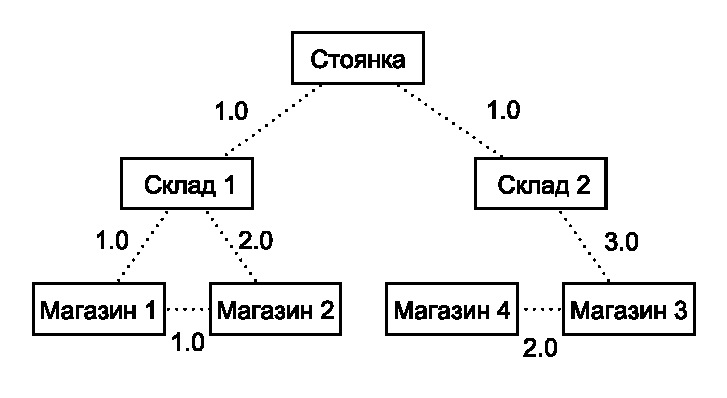
\includegraphics[scale=1.0, angle=0]{img/max_elem_1.pdf}}
			\caption{Начальное состояние системы}
			\label{pic:pre_1}
		\end{center}
	\end{figure}

	Пусть баланс задан таблицей \ref{init_balance}, объём тары $1.0 m^3$, вместимость грузовика $10.0 m^3$.
	
	\begin{table}[h]
		{\small \begin{center}
			\caption{Начальный баланс системы}
			\label{init_balance}
			\begin{tabular}{| p{5cm} | p{2.5cm} | p{2.5cm} |}
				\hline
				\backslashbox{\textbf{Пункт}}{\textbf{Продукт}} &
				A &
				B \\
				
				\hline
				Стоянка & 
				$0$ &
				$0$ \\
				
				\hline
				Склад 1 & 
				$+10$ &
				$+10$ \\
				
				\hline
				Склад 2 & 
				$+10$ &
				$+10$ \\
				
				\hline
				Магазин 1 & 
				$-8$ &
				$-3$ \\
				
				\hline
				Магазин 2 & 
				$-2$ &
				$-2$ \\
				
				\hline
				Магазин 3 & 
				$0$ &
				$-4$ \\
				
				\hline
				Магазин 4 & 
				$-4$ &
				$0$ \\

				\hline
			\end{tabular}
		\end{center}}
	\end{table}

	После обработки всех рёбер между магазинами и стоянками для системы будут составленны маршруты, обозначенные на рисунке \ref{pic:pre_2} с помощью стрелок. Порядок их назначения будет следующим:
	
	\begin{enumerate}
		\item Кратчайший путь Склад 1 -> Магазин 1. Для него назначается перевозка 8 тар товара А и 2 тары Б. Для оставшейся тары продукта Б выделяется ещё один рейс по этому же маршруту. Заказ магазина 1 выполнен, он исключается из рассмотрения.
		\item Следующий кратчайший путь Склад 1 -> Магазин 2. Назначается перевозка 2 тар продукта А и B.
		\item Последний путь Склад 2 -> Магазин 3. Назначается перевозка 4 тар продукта B.
	
	\end{enumerate}
	
	\begin{figure}[h]
		\begin{center}
			{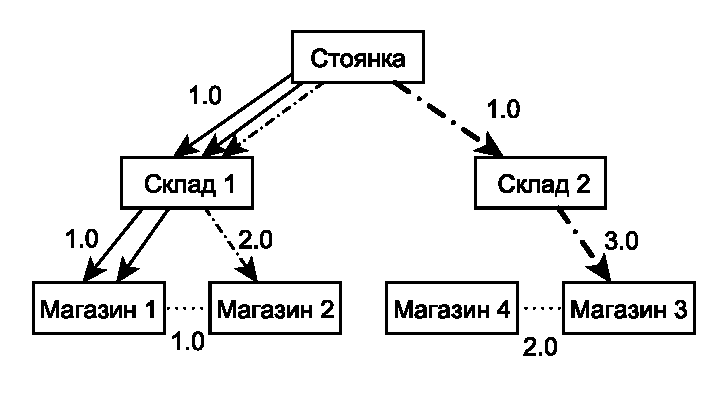
\includegraphics[scale=1.0, angle=0]{img/max_elem_2.pdf}}
			\caption{Начальное задания маршрутов}
			\label{pic:pre_2}
		\end{center}
	\end{figure}

	Так как остался Магазин 4 с неудовлетворённым заказом, из-за невозможности удовлетворить его потребностями непосредственно связанными с ним складами, для него осуществляется поиск расстояний до всех складов. Склад 2 расположен на расстоянии $5.0$, склад 1 -- $7.0$. Второй ближе, следовательно из него назначается перевозка на 4 тары продукта A. После этого потребности всех магазинов удовлетворены. Состояние системы после окончания предварительного этапа изображено на рисунке \ref{pic:pre_3}
	
 	\begin{figure}[h]
	 	\begin{center}
	 		{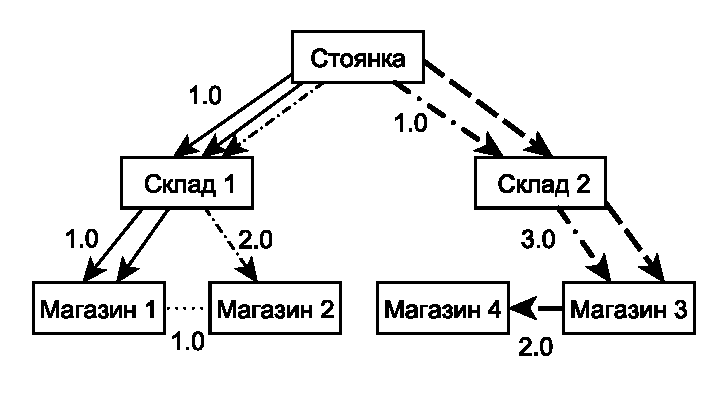
\includegraphics[scale=1.0, angle=0]{img/max_elem_3.pdf}}
	 		\caption{Система после дополнительного задания маршрутов}
	 		\label{pic:pre_3}
	 	\end{center}
	 \end{figure}
 
 	Если оценить состояние грузовиков, то можно отметить неоптимальность созданного плана. Грузоперевозку в магазин 2 можно осуществить на 2-м рейсе, так как в машина загружена неполностью, а удлинение маршрута будет дешевле назначения отдельного рейса. Аналогично совмещается грузоперевозка в 3 и 4 магазины. Поэтому созданный план требует дополнительную обработку.
	
	\paragraph{Основной этап}
	Основу алгоритма составляет метод потенциалов. Его целью является нахождение окончательного оптимального плана \cite{potential}. Действие заключается в следующем.
	
	Каждый узел обладает некоторым значением потенциала $Pot[P]$. Фактически оно отражает значение целевой функции для определённого пункта. Изначально оно задаётся в соответствии с сформированным на первом шаге плане. Значение складов устанавливается как стоимость проезда до стоянки. Значения для магазина $Pot[P_j]$ считается как $Pot[P_j] = Pot[P_i] + Cost_{ij}$, где $Pot[P_i]$ - потенциал пункта, из которого по плану осуществляется доставка груза, $Cost_{ij} = d_{ij}$ - стоимость перевозки груза по дуге $ij$.
	
	Оптимизация производится за счёт рассмотрения альтернативных путей доставки груза в пункт вместо уже запланированных. Это делается при помощи определения значения невязки для каждой дуги. Для пути $P[i] -> P[j]$ оно вычисляется как $-Pot[P_j] + Pot[P_i] + Cost_{ij}$. В случае, если данная величина отрицательна это фактически означает, что существует более выгодный маршрут перевозки. Производится пересчёт потенциалов и всех невязок. В случае, если все невязки положительны считается, что оптимальное решение найдено. Иначе, выбирается самая значительная невязка и для неё повторяется описанный шаг.
	
	Обратимся снова к выделенным дополнительным условиям задачи.
	\begin{itemize}
		\item Потенциал одного пункта зависит от маршрута, проходящего через этот пункт. Например, через один пункт может пролегать два маршрута. Стоимость доставки товара в первом является минимальной, если идёт по кратчайшему пути от нужного склада. Во втором она выше, так как до этого посещаются другие пункты. Значения потенциалов получаются разными, поэтому следует выбирать максимальных из них.
		\item Невязка дуги должна отражать то, что при замене доставки в данный пункт по иному маршруту, старый маршрут может перестать существовать. Поэтому невязка должна высчитываться как $-Pot[P_j] + + Cost_{ij}$. Данная величина равна изменению целевой функции в случае продления маршрута, идущего через $P_i$, и удаление через $P_j$.
		\item Значение потенциала также зависит и от рассматриваемого продукта. Если в пункт не ведёт ни один маршрут, который перевозит или потенциально может перевести некий продукт, то значение потенциала для данного продукта будет бесконечным. Поэтому для каждого товара рассчитываются собственные значения потенциалов. Значение невязки дуги считается минимальным среди невязок по всем продуктам.
	\end{itemize}

	Учтивая перечисленные нюансы следует скорректировать метод. Наличие отрицательной невязки означает, что из данного пункта, вероятно, возможна более выгодная перевозка взамен существующей. Следует осуществить проверку на соблюдение условий вместимости, наличия достаточного количества товара новом складе и т.д.. Поэтому при обнаружении отрицательной невязки оптимизируемый пункт лишь планируется к дальнейшему рассмотрению.
	
	После подсчёта потенциалов начинается анализ пунктов, к которым ведут дуги с отрицательной невязкой. Рассмотрение производится в порядке возрастания невязок. 
	
	При рассмотрении пункта составляется список всех маршрутов, которые могут пройти через дуги с невязкой. Альтернативные маршруты удлиняются до пункта и берут на себя максимальный объём продукции, который позволяет вместимость их транспорта и запасы на складе. Маршруты должны рассматриваться в порядке минимальной стоимости перевозки по ним продукции до данного пункта. Данную величину для $k$-го маршрута можно вычислить как $Cost_{ij} \cdot [Vol \cdot $\(\max\limits_{1 \leq i, j \leq N}\)$ (\sum_{l=1}^{N_{Prod}} v_{ijkl})]$. Поэтому, маршруты без свободного места рассматриваться не будут вне зависимости от их близости к пункту. 
	
	Когда вся продукция рассматриваемого маршрута была перераспределена на другие находится значение функции оптимизации $L$ и сравнивается с исходным. Если новое значение ниже, значит новые маршруты более оптимальные, чем старые. Они принимаются за исходный план и процесс оптимизации переходит к следующей итерации.

\subsection{Метод составления расписания}
После формирования оптимальных маршрутов перевозок для завершения планирования остаётся решить задачу назначения транспорта на каждый маршрут, а также выбора времени начала каждой перевозки. Составление расписания должно руководствоваться следующими соображениями.

\begin{itemize}
	\item Время завершения каждого маршрута не должно превосходить время окончания рабочего дня водителей.
	\item Один транспорт не может одновременно находится сразу на нескольких маршрутах.
	\item При составлении плана желательно избегать ситуаций, когда несколько машин одновременно будут грузиться на одной и той же точке маршрута. Это обусловленно тем, что в таком случае нельзя гарантировать, что время обслуживания грузчиками двух и более грузовиков, оказавшихся в одном месте останется неизменным ввиду возможного падения скорости погрузки.
\end{itemize}

Данная задача может быть решена с использованием метода интервалов \cite{schedule:intervals}, где пункты погрузки рассматриваются как ресурсы, которые могут быть использованы одновременно только в одном интервале. Действие метода заключается в следующем.

Изначально для каждого маршрута рассчитывается время прибытия и отбытия для каждого пункта. У всех маршрутов на этом этапе время начала принимается минимальным возможным, то есть временем начала рабочего дня $t_{begin}$.

На одну из машин назначается произвольный маршрут. Время начала и завершения фиксируются в расписании. Выбор маршрута влияет на дальнейшее составление расписания, и может оказаться не самым оптимальным по критерию времени завершения последнего рейса. Но также не стоит и задачи оптимизации по этому параметру -- он должен не превосходить $t_{end}$. В случае, если в результате планирования это условие не выполняется, метод будет использован заново, но с иным выбором первого маршрута.

Далее просматривается список нераспределенных маршрутов. Из него выбирается маршрут с минимальным временем начала. Он сравнивается с маршрутами из расписания на предмет наличия коллизий -- пересечения интервалов погрузки на одинаковых пунктах. В случае, если таковых не найдено, он помещается в расписание с фиксированием транспорта и временем посещения пунктов. 

Если коллизия найдена, то время начала рассматриваемого маршрута увеличивается так, чтобы её избежать, после чего он возвращается в список нераспределенных маршрутов. 

Действие повторяется до тех пор, пока все маршруты не окажутся в расписании.

\pagebreak